\begin{multicols*}{3}
\setlength{\premulticols}{1pt}
\setlength{\postmulticols}{1pt}
\setlength{\multicolsep}{1pt}
\setlength{\columnsep}{2pt}

\subsection{1. Getting Data}
\subsubsection{1.1, 1.7 Exploratory Data Analysis and Studies}
\textbf{Population}: Entire group to to reason about.\\
\textbf{Research Question}:  Investigate a characteristic of a population, should be \underline{Less Narrow, Focused, \& Complex}.\\
\textbf{Exploratory Data Analysis}:
\begin{enumerate}
    \item Generate a research question.
    \item Collect and Model Data.
    \item Draw conclusions about the data.
    \item Refine or create new questions if necessary.
\end{enumerate}
\textbf{Experimental Study}: Controlled manipulation of independent variables to provide evidence of cause and effect relationship. Random assignment and Single/Double Blinding help to reduce placebo effect and researcher bias.\\
\textbf{Observational Study}: Measures variables of interest without manipulation, provide correlation information only. Used when conducting an experiment is not feasible.


\subsubsection{1.2 Sampling}
\textbf{Population Parameter}: Numerical fact about the population.\\
\textbf{Sample}: A subset of the population of interest.\\
\textbf{Sampling Frame}: Set from which a sample is drawn.\\
\textbf{Census}: Sample the entire population.\\
\textbf{Probability Sampling:} Random selection, every unit of the sampling frame has a \underline{known non-zero}(not necessarily same) probability.
\begin{itemize}
    \item \textbf{Simple Random Sampling}: Random selection with equal probability for all units. Good representation but time-consuming.
    \item \textbf{Systematic Sampling}: Sample every k units, with k determined randomly. Easy but potential under-representation if there is inherent order to data.
    \item \textbf{Stratified Sampling}: Randomly select from each stratum k units, with k proportionate to size of stratum. Good representation per stratum but requires clear criteria to divide the sampling frame.
    \item \textbf{Cluster Sampling}: Divide frame into clusters, and randomly pick 1 whole cluster. Extremely easy but requires clusters to be representative of the population.
\end{itemize}
\textbf{Non-Probability Sampling:} Units are selected by discretion.
\begin{itemize}
    \item e.g. Convenience Sampling, Volunteer Sampling
\end{itemize}
\textbf{Selection Bias}: Parts of the population being excluded from the sampling frame. can be caused by imperfect sampling frame or non probability sampling.\\
\textbf{Non-response Bias}: Exclusion dude to non disclosure/response of sample participants. Occurs regardless of sampling method.\\
\textbf{Generalisability Criteria}: Sampling Frame $\subseteq $ population, probability sampling, large sample size, minimize non response rate.

\subsubsection{1.3-1.6 Variables and Summary Statistics}
Manipulate \textbf{Independent} variables and measure changes in \textbf{Dependent} variable.\\
\textbf{Categorical} variables take on mutually exclusive labels. Arithmetic operations have no meaning
\begin{itemize}
    \item \textbf{Nominal} variables have no intrinsic ordering.
    \item \textbf{Ordinal} variables have an intrinsic ordering.
\end{itemize}
\textbf{Numerical} variables take on values, and arithmetic operations have meaning. Can be \textbf{Discrete} or \textbf{Continuous}.\\
\textbf{Mean}: $\bar{x}=\frac{1}{n}\sum x_i$; \textbf{Variance}: $s^2=\frac{1}{n-1}\sum(x_i-\bar{x})$; \textbf{Std Dev}: $s$\\
\textbf{Mode}: most frequently appearing value(s); \textbf{Q1}, \textbf{Median}, \textbf{Q3}: $X_{(n*p)}$ or $\frac{1}{2}(X_{(n*p)} + X_{(n*p + 1)})$ for $p=0.25, 0.5, 0.75$; \textbf{IQR}: $\text{Q3}-\text{Q1}$; Outliers are outside $[\text{Q1}- 1.5 \times \text{IQR}, \text{Q3}+ 1.5 \times \text{IQR}]$\\

\subsection{2. Categorical Data Analysis}
\subsubsection{2.1 Rates}
$P(X\cap Y) = P(X|Y)\cdot P(Y)=P(Y|X)\cdot P(X)$\\
\textbf{Positive Association} when $P(X|Y)> P(X|Y')$ or $P(X'|Y')> P(X'|Y)$ and \textbf{Negative Association} when $<$.\\
\textbf{Symmetry Rule}:  $P(X|Y)> P(X|Y') \Leftrightarrow P(Y|X)> P(Y|X')$.\\
\textbf{Basic Rule}: $P(X)\in [P(X|Y), P(X|Y')]$.\\
\textbf{Simpon's Paradox} occurs when a trend present in $\gt$ half the groups of data disappears when the groups are combined.\\
A \textbf{Confounding Variable} is uncontrolled and associated with both the independent and dependent variables.\\
Include confounders as independent variables or use random assignment to reduce impact.

\subsection{3. Dealing with Numerical Data}
\textbf{Data Distribution} can be described by no. of peaks(shape), skewness(center) and variance(spread).
\begin{center}
    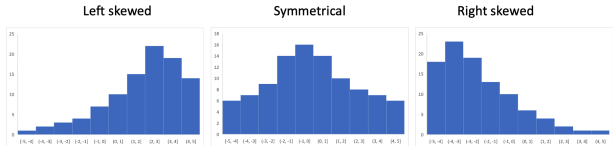
\includegraphics[width=1\linewidth]{cheatsheet/skewness.png}
    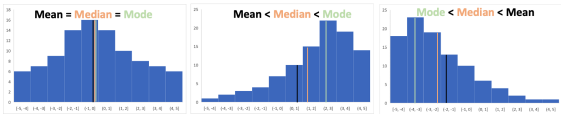
\includegraphics[width=1\linewidth]{cheatsheet/central_tendency.png}
\end{center}
Relationships can be linear/non-linear and its strength is based on closeness to the predicted value. \\
\textbf{Correlation} $\subset$ association, is a linear relationship between 2 variables. \textbf{Correlation Coefficient}, $-1\leq r \leq 1$, measures the direction and strength. r is reflexive and invariant to scaling and translation.\\
\begin{center}
    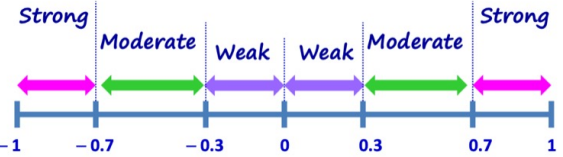
\includegraphics[width=0.7\linewidth]{cheatsheet/correlation_strength.png}
\end{center}
r does not imply causation, does not show non-linear association and is greatly affected by outliers.\\
\textbf{Ecological Fallacy}: Drawing conclusions about individuals/subsets based on the aggregate. \textbf{Atomistic Fallacy} is the vice versa.
\textbf{Linear Regression} uses least squares error, $e=(\hat{y_i}-y_i)^2$, to fit the regression line $\hat{y}=mx+c$, $m=\frac{s_y}{s_x}r$ to predict the average $\hat{y_i}$ for a given $x_i$. The regression line always contains $(\bar{x}, \bar{y})$.

\subsection{4. Statistical Inference}
The \textbf{Sample Space} contains all possible \textbf{Outcomes}, a \textbf{Event} is a subset of the sample space.
$P(S) = 1$; $0\leq P(E)\leq1$; Mutual Exclusion is $P(E \cup F)=P(E)+P(F)$; Independence is $P(E\cap F)=P(E)\cdot P(F)$.\\
\textbf{Law of Total Probability}: $P(G)=P(G|E)\cdot P(E)+P(G|F)\cdot P(F)$ if $E$ and $F$ are mutually exclusive.\\
\textbf{Prosecutor's Fallacy} is confusing $P(A|B)$ and $P(B|A)$.\\
\textbf{Conjunction Fallacy} is believing $P(A\cap B)$ $>$ $P(A)$ or $P(B)$.\\
\textbf{Base Rate Fallacy} is drawing conclusions about a conditional without factoring in the base rate of the condition.\\
\textbf{Sensitivity} is the true positive rate. \textbf{Specificity} is the true negative rate.\\
$\text{Sample Statistic}=\text{Population Statistic}+\text{Bias}+\text{Random Error}$\\
A \textbf{$\alpha\%$ Confidence Interval} has $\alpha\%$ confidence of the population statistic being included in the interval, or that $\alpha\%$ of confidence intervals constructed from samples of the same size will include the population statistic.\\ 
Proportion CI: $\hat{p}\pm Z\sqrt{\frac{\hat{p}(1-\hat{p})}{n}}$, t CI $\bar{x}\pm t\frac{s}{\sqrt{n}}$. The margin of Error is $Z\sqrt{\frac{\hat{p}(1-\hat{p})}{n}}$ or $t\frac{s}{\sqrt{n}}$.\\
A $\alpha$ significance level \textbf{Hypothesis Test} checks if we reject the null hypothesis $H_0$ with $\alpha$ probability of a Type I error (Rejecting $H_0$ when it is true). The test statistic is $\frac{\hat{p}-p_0}{\sqrt{\frac{\hat{p}(1-\hat{p})}{n}}}$ and $\frac{\bar{x}-x_0}{\frac{s}{\sqrt{n}}}$.
\begin{center}
    \centering
    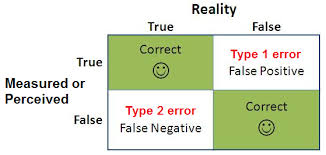
\includegraphics[width=0.5\linewidth]{cheatsheet/type1-2_errors.png}
\end{center}
\end{multicols*}